\documentclass{article}
\usepackage{amsmath}
\usepackage{graphicx}
\usepackage{siunitx}
\usepackage{float}
\usepackage{gensymb}
\usepackage[dvipsnames]{xcolor}
\usepackage{sectsty}

%\setlength{\parskip}{1em}

%\definecolor{color:background}{RGB}{40,40,40}
%\definecolor{color:text}{RGB}{230,230,230}

%\pagecolor{color:background}
%\color{color:text}
\allsectionsfont{\normalfont\sffamily\bfseries}

\title{ELEC 344 Lab Report 4}
\author{Kelvin Hsu 46308152\\ Alex Lim 47049151\\ Matthew Chan 52416154}


\begin{document}
    \sffamily
   	\maketitle
    \newpage

    \section*{5A-1)}
    $R_{1}$ and $L_{m}$ can be found using the no load test where $S \sim 0$ and rotor circuit can be treated as 
    open circuit.
    \subsection*{Calculating $R_{1}$}
       \begin{align*} 
            &P_{nl} = I_{rms}V_{rms}cos(\theta)\\
            &\boxed{R_{1} = \frac{P_{nl}}{I_{rms}^{2}}/2 = 0.345/2 = 0.1725 \ohm}
       \end{align*}

    \subsection*{Calculating $L_{m}$}
       Assuming $L_{m} \gg L_{l1}$.
       \begin{align*}
            &P(\text{Reactive Power}) = \sqrt{I_{rms}^{2}V_{rms}^{2} - P_{nl}^{2}} = \omega*L_{l1}*I_{rms}^{2}\\
            &\omega = 2 \pi 60Hz\\
            &\boxed{L_{lm} = 0.0086529H}
       \end{align*}
    \subsection*{Calculating $L_{l1}$, $L_{l2}$, and $R_{2}$}
    $L_{l1}$, $L_{l2}$, and $R_{2}$ can be found using block motor test.
    Assuming the impedance of $L_{l2}$ in series with $R_{2}$ is much smaller than the impedance of $L_{m}$.
       \begin{align*}
            &\boxed{R_{2} = \frac{P_{total}/3}{I_{rms}^{2}} = 0.2839\ohm}\\
            &(L_{l1} + L_{l2})\omega I_{rms}^{2} = \sqrt{(V_{rms}^{2}I_{rms}^{2}) - (P_{total}/3)^{2}}\\
            &\boxed{L_{l1} = L_{l2} = 0.000731913H}
       \end{align*}

    \subsection*{Calculating Number of Poles}
       \begin{align*}
            &\text{motor rpm} = \frac{120f_{in}}{p}\\
            &p = 120*60/1750 = 4.11 \sim 4
       \end{align*}

    \subsection*{Calculating Power Factor}
       \begin{align*}
            &\omega_{synchronous} = 0.5 * 2 * \pi * 60 = 188.495 rad/s\\
            &\omega_{rotor} = 1750rpm * 2\pi / 60 = 183.259 rad/s\\
            &\omega_{slip} = 5.23598 rad/s\\
            &\theta = tan^{-1}(\frac{\omega_{slip}L_{l2}}{R_{2}}) = 0.77335 \degree\\
            &cos(\theta) = 0.9999
       \end{align*}
    \section*{5A-2}
    From Table-6, $R_{2}$ is estimated. Looking at the table, the first and the 4th measurements are outliers.
    The 2nd and 3rd give the best estimate of $R_{2}$ because the slip is smaller relative to the later measurements.
    The estimate is also really close the the resistance calculated in 5A-1.
    \begin{equation*}
        R_{2} = 0.32\ohm
    \end{equation*}

    \section*{5B:Equivalent Circuit vs Measured Comparison}
    From the equivalent circuit, we found the Thevenin Equivalent treating the rotor circuit as load such that 
    rotor current can be found.

    Python script is used to calculate the Thevenin equivalent parameters.
    
    \begin{align*}
        &V_{th} = 17.95788\\
        &Z_{th} = 0.14699 + 0.262784j\\
        &I_{rotor} = V_{th}/Z_{total}\\
        &Z_{total} = 0.14669 + R_{rotor}/s + (0.262784 + X_{l2})j \\
        &P_{em} = 3*I_{rotor}^{2}*R_{rotor} * (1-s) / s \\
        &T_{em} = P_{em} / \omega_{rotor}
    \end{align*}

    \begin{figure}[H]
        \centering
        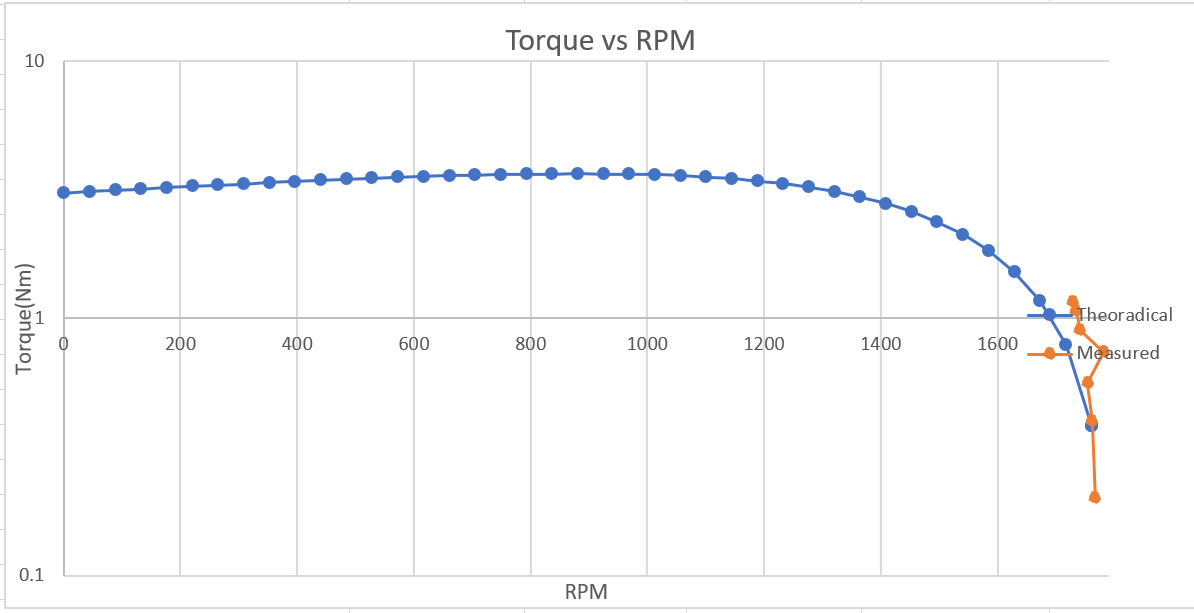
\includegraphics[width=12cm, height = 8cm]{figures/rpm_torque.PNG}
        \label{fig:rpm_torque}
    \end{figure}

    \begin{figure}[H]
        \centering
        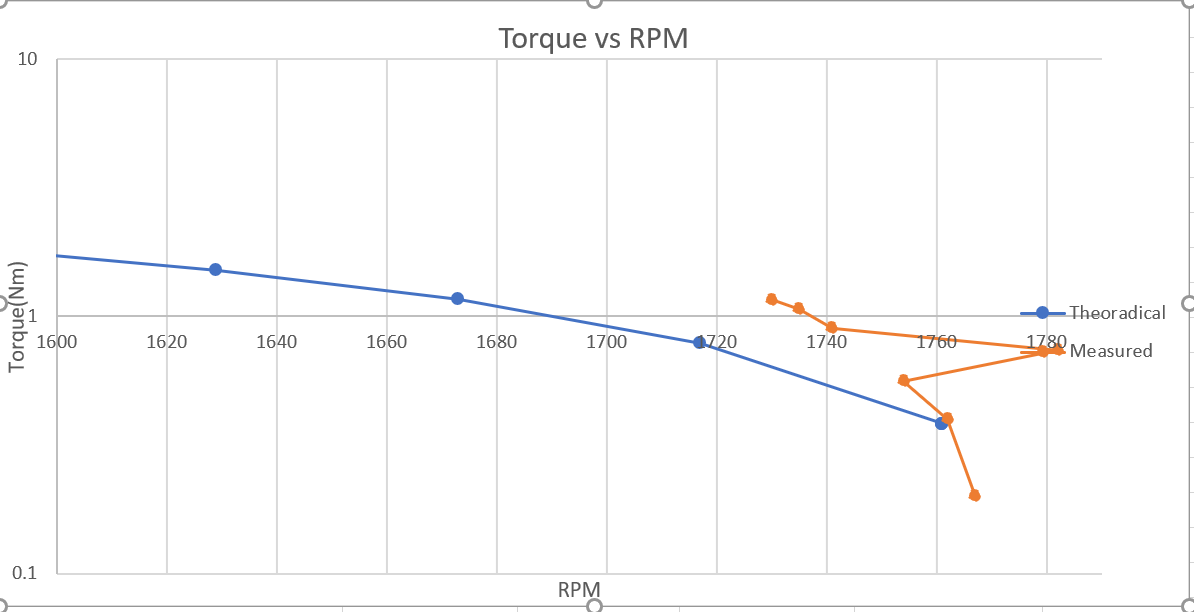
\includegraphics[width=12cm, height = 8cm]{figures/rpm_torque_zoom_in.PNG}
        \label{fig:rpm_torque_zin}
    \end{figure}

    As shown in the graphs, the measured values starts to decrease just before the theoretical 
    reaches the pull out torque and start decreasing. Ideally both graph should reach 0 torque at 1800 rpm 
    since s will approach 0.




    
    

            
        


        

\end{document}

 